
\section{Introduction}
	YoMap Matlab is an open source mapping application for city Le Creusot. It was developed as a Software Engineering final project by a group of ViBOT/MsCV students using C++, Qt, OpenGL and Boost library. YoMap contains the basic data and functions that can help you to get around the city. In this user manual you will find detailed instructions of how to use Yomap.
	
For any questions free welcome to contact:
Ozan: emreozanalkan@gmail.com
Klemen: 
Oksana:
Natalia: natalia.shepel@gmail.com
\begin{center}
Enjoy!
\end{center}

	
\section{Getting Started}
	The opened application window can be seen on figure 1. Main elements of map:
	\begin{enumerate}
		\item Search Panel
		\item Map
	\end{enumerate}
	
	 \begin{figure}[h]
	 \centering
	 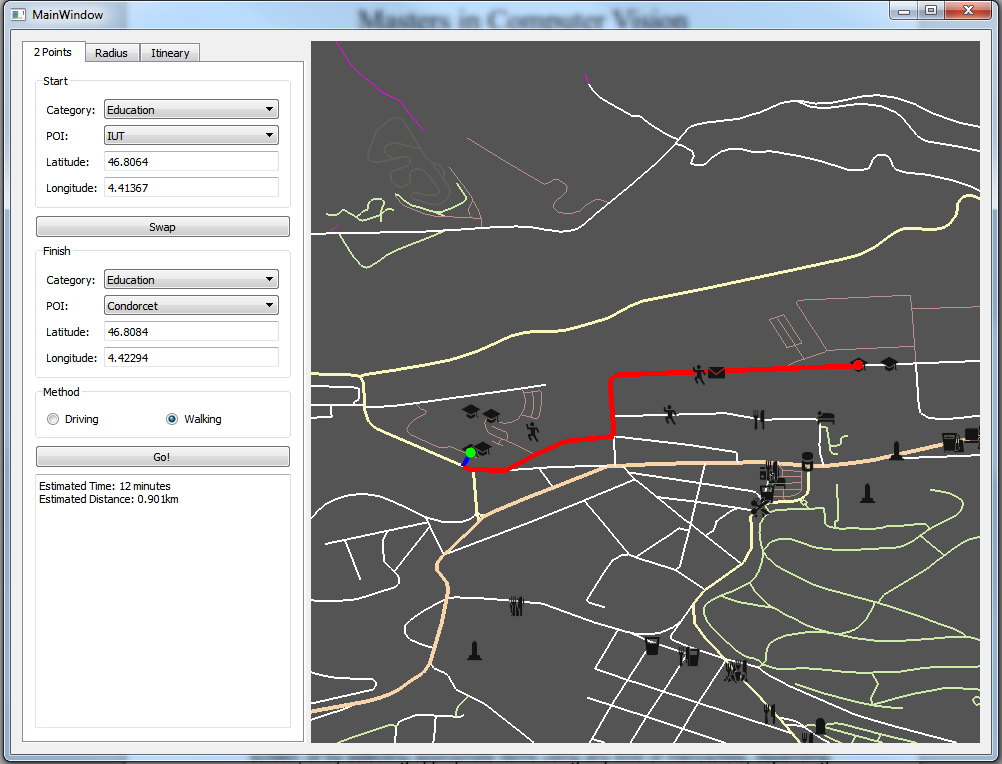
\includegraphics[ width=\textwidth]{2point_0.png}
	 \caption{Basic view of the application}
	 \end{figure}
	
	To move the map, hold right click on the map and drag the map. To zoom in or zoom out use scroll on your mouse or touch pad.
	
	To view details about the point of interest right click on corresponding icon. 
	
	To centre the map click "c" or left click on the map and select "Center the map" in the context menu.
		
\section{Data Entry}
	There are three options to enter the start or finish point.
	\subsection{By mouse click} Left click on the mouse and chose "Set starting point" or "Set ending point" in the context menu. Coordinates of the clicked point will appear in the text fields on the left.
	\subsection{By coordinates} Enter the geographical coordinates in the corresponding text fields on the left.
	\subsection{By POI} First choose the category in the Search panel ComboBox on the left. Then select the POI in the similar way.	
	Use "Swap" button to switch the data between the start and finish points.	

\section{Point of Interest Add/Edit}
	To add new point of interest please left click on the map and select "Add as a POI" in the context menu. Then enter Name and Category to the Dialogue that appears. To save data click "Save", otherwise click "Cancel". 
	To edit POI right click on the POI, you want to edit. Then click button "Edit" in the small window that appears. Edit the fields you need and press "Save" to save and "Cancel" to cancel changes.

\section{Shortest Path Search}
	To find shortest path between 2 points chose the first tab in the Search Panel. Enter start point and finish point in any of the ways described above and press "Go!" button. All information about time and distance will appear on the bottom of the Search Panel and path will be shown on the map.
	
\section{Radius Search}
	To find closest object to initial point from category press the "Radius" tab on the top of the Search Panel. Enter information for start point and choose the category of POI you want to search in the given radius. Use slider or text box to enter the maximum radius of the search in meters. Note, that 0 distance corresponds to unlimited distance search. Press button "Go!". All the possible ways will be shown on the map and printed in the text field on the bottom of the Search Panel.

\section{Shortest Path Search With Middle Points}
	To find path with a middle point click on the "Itinerary" tab on the search panel. Enter information for start and end point and choose category from the menu of middle point. You can add up to three intermediate categories. To add new point use "Add Point", to delete use "Delete Point". Use slider or text box to enter the maximum radius of the search in meters. Press button "Go!". The path with the required middle point will be chosen.
	